\section{REVIEW OF LITERATURE}

\subsection{Overview}

This section reviews the related literature through a systematic review, which identifies, screens, and selects studies by a documented and repeatable procedure rather than by narrative selection. A narrative review reports what a few chosen studies do, but it cannot show what the field as a whole has left undone, and a new model must be justified against that undone work. A systematic procedure makes both the body of studies retained for analysis, hereafter the corpus, and the research gap it reveals defensible.

The review concerns agent-based models (ABMs), simulations in which individual entities such as pests, crops, and farmers are represented as interacting agents, applied to insect pest management. It addresses three questions. First, what agent-based models exist for insect pest management, and how are they built? Second, along the dimensions that matter for a soft-scale model on sugarcane, how is the field distributed, and which modelling options are common, rare, or absent? Third, where in that distribution does a model of RSSI fall, and what does it contribute that no reviewed model provides?

\subsection{Review Method}

The review followed the PRISMA 2020 guidelines \citep{Page2021} for identification, screening, and selection, so the path from raw records to the final studies is logged and reproducible. The analytical organisation, described in the next subsection, codes each study against published typologies of model structure, agent architecture, and validation \citep{Taillandier2019,Wooldridge1995,Rykiel1996}.

The search covered two databases, Web of Science and Scopus. The query combined three concept blocks: a modelling-method block (agent-based, individual-based, multi-agent), a pest-and-management block, and an agricultural-context block. The same finalised string was run in both databases, differing only in field-tag syntax (Web of Science TS=, Scopus TITLE-ABS-KEY), with no date or document-type filters.

The two databases returned 426 records, 125 from Web of Science and 301 from Scopus. Removing 117 duplicates left 309 unique records. Title-and-abstract screening excluded 262 records and selected 47. The inclusion criterion required a record to describe an agent-based or individual-based model of an insect pest and its management in an agricultural or comparable setting. Full-text review of the 47 excluded 17 further studies and retained 30. Table~\ref{table:exclusions} categorises every exclusion against that single criterion. The 262 abstract-screening exclusions fall into four types: records off-topic on an incidental keyword match, such as materials-chemistry, life-cycle-assessment, and remote-sensing papers (about 39\%), studies of a system that is not an insect crop-pest, such as birds, livestock, weeds, or disease vectors (about 36\%), relevant insect-pest agent models too thin to warrant full-text review (about 19\%), and pest studies using a non-agent method, such as a statistical risk index or a differential-equation population model (about 5\%). The largest full-text exclusions are reviews rather than primary models and studies whose model focus is out of scope, such as resistance genetics or beneficial-insect dynamics. A third group is redundant restatements of one wind-borne aphid dispersal model, of which two were kept to represent it \citep{Wang2019,Koralewski2022} and four close repeats were dropped. The remaining exclusions are software or educational models and one non-agent reaction-diffusion model. Each final study carries its source database, duplicate status, screening decision and reason, full-text decision, and analytical codes, so the funnel from 426 to 30 can be audited.

\begin{table}[!htbp]
\vspace{2ex}
\centering
\caption{Exclusion categories against the single inclusion criterion (an agent-based or individual-based model of an insect crop-pest and its management).}
\label{table:exclusions}
\begin{tabular}{llr}
\hline\hline
Stage & Exclusion type & Count \\ \hline
Abstract (262) & Off-topic incidental keyword match & about 39\% \\
 & Not an insect crop-pest system & about 36\% \\
 & Relevant pest ABM, too thin for full text & about 19\% \\
 & Not an agent-based method & about 5\% \\
Full text (17) & Review or synthesis, not a primary model & 5 \\
 & Out-of-scope focus & 5 \\
 & Redundant restatement of a retained aphid model & 4 \\
 & Software package or educational model & 2 \\
 & Not an agent-based or individual-based model & 1 \\ \hline\hline
\end{tabular}
\vspace{2ex}
\end{table}

\begin{figure}[!htbp]
\begin{center}
	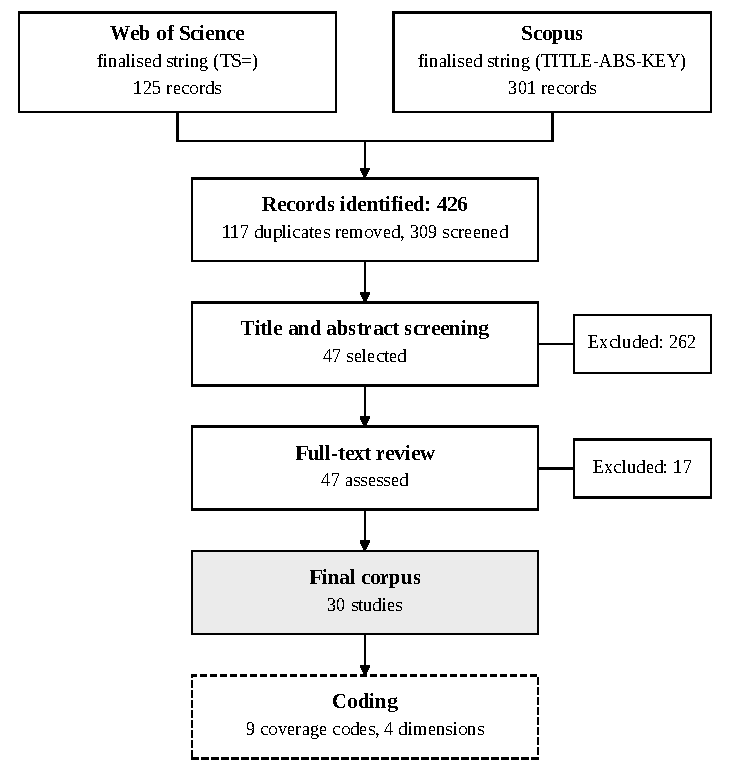
\includegraphics[width=0.9\textwidth]{figures/fig-slr-flow}
	\caption{Flow of the systematic review, from 426 database records through duplicate removal, abstract screening, and full-text review to the 30 final articles.}
	\label{fig:slrflow}
\end{center}
\end{figure}

\subsection{Analytical Framework}

Each of the 30 final studies was coded in two ways. The first is a set of nine coverage codes recording, for each study, the presence or absence of a feature relevant to an RSSI model: a reusable ABM structure, control-strategy testing, model validation, damage-to-yield coupling, temperature or weather drivers, spatial spread, biological control, chemical control, and a farmer decision agent. These codes record whether the field has addressed each component the proposed model needs.

The second is a set of four analytical dimensions. Each dimension takes a published typology together with its full set of values, so a value that no study occupies appears as an empty cell. Spatial representation uses the environment topologies available in the GAMA platform as catalogued by \citet{Taillandier2019}: grid, graph, and continuous. The grid is split by georeferencing. An abstract grid, a schematic lattice of placeless cells, is distinguished from a raster, the same cells tied to a real landscape through a GIS layer, because an RSSI model of actual Negros fields needs the georeferenced kind. A non-spatial value covers models with no explicit environment. Agent architecture uses the reactive, deliberative, and hybrid distinction of \citet{Wooldridge1995}. Validation type uses the distinction between output validation, in which simulated outputs are matched to observed data, and structural validation, in which the model's mechanisms are checked, for example by experts or stakeholders \citep{Rykiel1996}. The farmer decision dimension uses a scheme defined from the corpus, separating behavioural, economic-optimisation, and empirical-rule models from studies with no farmer agent. Coding the corpus against fixed, externally defined value sets records where the field is dense and where it is empty.

Host crop, pest taxonomic group, and modelling platform are recorded as descriptors. The crop labels a study but does not distinguish a modelling choice, so it is reported in the corpus characterisation that follows.

\subsection{The Corpus}

The 30 studies confirm that agent-based pest modelling is an established genre. All 30 carry a reusable ABM structure, which follows from the inclusion criterion. Spatial spread is represented in 21 studies, model validation in 20, and control-strategy testing in 18, so the field is well developed on where a pest is, how it moves, and whether the model was checked. Temperature or weather drivers appear in 15 studies and a damage-to-yield coupling in 12. The two control levers this study contrasts are each present in about a third of the corpus, biological control in 11 studies and chemical control in 9. The least common feature is a farmer modelled as a decision agent, in 8 of the 30.

Sugarcane is a minority setting. Of the 30 studies, five model sugarcane \citep{Alves2024,Alves2026,vanVuuren2018,Human2023,Potgieter2025}, and all five model stalk borers or a weevil. Tree or fruit crops account for 5 studies, field or row crops for 14, and 2 are set outside a cropping system. The remaining 4 are generic. The pest taxonomy is the decisive descriptor. Lepidopteran borers and miners account for 10 studies, Coleoptera for 3, mobile hemipteran sap-suckers such as whitefly, aphid, and lanternfly for 6, Diptera for 2, Orthoptera for 1, and plant disease for 2, with 6 focused generically on natural enemies or farmer behaviour. No study models a scale insect of the superfamily Coccoidea, the group that contains RSSI. The nearest modelled hemipterans are mobile, and RSSI is sessile.

Platforms concentrate on NetLogo, named in 13 of the 30 studies. A further 13 studies used other named environments, including AnyLogic \citep{vanVuuren2018}, Python \citep{Human2023,Potgieter2025}, Delphi \citep{Gergs2026}, MPMAS \citep{Grovermann2017}, and CORMAS \citep{Rebaudo2011,RebaudoDangles2011}. The remaining 4 named no platform. No reviewed study uses GAMA.

The closest precedents to the proposed model cover the two halves of what an RSSI management model needs. \citet{Alves2026} modelled the sugarcane weevil \emph{Sphenophorus levis} in NetLogo. Their model coupled pest density to crop damage through a function that converted biomass loss to a percentage field loss and then to a monetary loss per hectare, switched development between two climate periods defined by local temperature and precipitation, and compared biological-control schemes against an uncontrolled baseline. It supplies the damage-function and economic side on the correct host crop, for a borer and with no farmer agent. For the spatial and validation side, \citet{Koralewski2022} and \citet{Wang2019} modelled the sugarcane aphid as an area-wide, weather-driven dispersal process on a gridded landscape and evaluated the forecasts against infestation observations. None of these models a scale insect, none uses GAMA, and none gives the farmer a decision. Between them they show that the damage-coupling, weather, spread, and validation components the proposed model needs have precedent in the corpus.

Two further models, outside the corpus, illustrate techniques relevant here. \citet{Anderson2015} modelled the spread of the emerald ash borer in a GIS-integrated Repast environment, calibrated against an observed rate of spread and validated against infestation records with 72\% spatial agreement, a clear example of output validation on spatial data. \citet{Wang2015} represented insect distribution within the plant at the leaf and canopy scale, an analogue to RSSI's leaf-position preference. Neither met the agricultural-context search criteria that define the corpus. The first is a forest pest and the second is a conference paper on within-plant behaviour.

\subsection{Synthesis}

Reading the corpus through the four dimensions shows a field concentrated in a few conventional choices and thin or empty elsewhere.

Spatially, 23 of the 30 studies use a grid, 17 abstract patch grids and 6 georeferenced rasters, which is the native representation in GAMA. Grids were used at scales from a single 1-ha field divided into cells \citep{Alves2024} to a region of about 1,750,000 km$^2$ divided into cells of 0.5$^{\circ}$ latitude by 0.5$^{\circ}$ longitude carrying crop and weather attributes \citep{Wang2019}. Continuous space appears in two studies, the locust hopper-band model of \citet{Bernoff2020} and the \emph{Eldana} model of \citet{vanVuuren2018}. A graph or network appears in one study, the multi-pathway spread model of \citet{McNitt2019}. The remaining four studies are non-spatial \citep{Grovermann2017,Gergs2026,Herbillon2024,Chen2024}. Every topology in the typology has at least one example. The single network model used a coarse trade-pathway graph linking regions and did not represent the field-to-field connectivity that cane cutting and haulage involve, so that application remains open.

In agent architecture, 22 of the 30 models are reactive. Pests and natural enemies respond to the current state of their environment without internal plans. Deliberative and hybrid architectures appear only in the 8 studies that model a farmer: one deliberative optimisation model \citep{Grovermann2017} and seven hybrid behavioural models, among them the Rebaudo and Pacilly studies, \citet{Bourceret2024}, and \citet{Chen2024}. The more developed decision machinery in the field is confined to the farmer side and has not been joined to a detailed pest-biology model.

Validation concentrates on the output type. Output validation was done in 16 studies, for example evaluating area-wide dispersal forecasts against infestation observations \citep{Koralewski2022}, validating a whitefly model against field-trial data from several locations in India \citep{Gergs2026}, and checking a fall-armyworm model against county field data \citep{Garcia2019}. Structural or participatory validation appears in 4 studies, including the expert-entomologist review of \citet{Potgieter2025} and the farmer workshops of \citet{Pacilly2019b}. A further 10 studies reported no validation beyond internal sensitivity analysis. Output validation on field data is the mainstream route, and a participatory or face-validation check is uncommon.

The farmer decision dimension is the sparsest. Of the 30 studies, 8 model a farmer decision agent: 6 behavioural, 1 economic-optimisation, and 1 empirical-rule. The behavioural models grounded the decision in a social or diffusion theory, as in the information-diffusion and cooperation models of \citet{Rebaudo2011}, \citet{RebaudoDangles2011}, and \citet{Rebaudo2013}, and the social-ecological model of \citet{Pacilly2019a}. The economic-optimisation model maximised a farm objective function under constraints \citep{Grovermann2017}. The empirical-rule model derived decisions from observed grower behaviour \citep{Chen2024}. The other 22 studies have no farmer agent and treat control as an externally set scenario.

Both control levers are modelled, usually one at a time. Biological control was represented as a natural-enemy or parasitoid mechanism \citep{vanRoermund1997,Collard2018,Delattre2019} or as a sterile-insect or microbial scheme \citep{Diouf2022,Herbillon2024}. Chemical control appeared as spraying regimes or pesticide-use accounting \citep{Grovermann2017}. An explicit comparison of a biological option against a chemical option, scored as a single decision, is uncommon in the corpus.

\subsection{The Research Gap}

The review locates three gaps, stated in decreasing order of how firmly the corpus establishes each one.

The first is the absence of a scale-insect model. No study among the 30 models a scale insect, whose crawlers settle on the host to feed \citep{Guerrero2026}, and the five sugarcane studies all model a borer or a weevil. There is no agent-based model of RSSI, or of any soft scale, on sugarcane, and none validated on Philippine or Negros field data. The nearest modelled hemipterans, cotton whitefly, sugarcane aphid, and spotted lanternfly, are mobile. Sessility is the decisive difference for a model. In an agent-based pest model, movement and spatial spread are core agent behaviours, and a scale insect disperses only briefly as a first-instar crawler before settling permanently on the plant, so dispersal rules written for a mobile whitefly or aphid do not carry over. A model of RSSI must be built new rather than reparameterised from an existing one.

The second is a structural gap at the intersection of the coding dimensions. Of the 30 studies, 8 model a farmer decision and 11 model biological control. No single study couples a farmer decision with both a biological-control option and a pest-biology component. The nearest study, \citet{Chen2024}, gave farmers a choice between biological and chemical control and carried no pest-biology component. The studies that couple a farmer decision to a pest-biology component, such as \citet{Grovermann2017}, modelled only chemical control. This claim rests on the per-study codes rather than on a single tabulated value.

The third concerns methods the field underuses. The single network model represents a coarse regional trade graph and leaves the field-to-field connectivity relevant to cane transport unaddressed. Although grids dominate the corpus, only 6 of the 30 studies use a georeferenced grid whose cells map to a real landscape. Structural or participatory validation is rare, in 4 of the 30 studies.

\subsection{Positioning of This Study}

The proposed model contributes on four points, each located in an empty or thin region of the review. It models RSSI, a scale insect absent from the corpus, on sugarcane, a crop present in 5 of the 30 studies. It gives the farmer a choice between biological and chemical control on top of a pest-biology model, a combination no reviewed study provides. It is implemented in GAMA, a platform no reviewed study uses, on a georeferenced grid of the actual Negros cane landscape, a representation used by only 6 of the 30 studies. Because no Negros infestation time series was found \citep{SRA2026FOI,PGNO2026}, its validation is limited to a hindcast against one verified observation (see Methodology), and output validation on field data is deferred until such data become available.
